\chapter{Compute the diameter}
\section{Definition of diameter}
The diameter is the maximum distance between two vertices
\section{A simple approach}
In the general case the best approach is calculate APSP (All Pairs Shortest Path) then find the maximum distance, that has a time complexity of $ O(n^{2.38}) $ where the 2.38 derive from some optimization on matrix calculation(see below) for dense graph while $ O(mn) $ for sparse graph. The problem with this simple approach is that is not usable in real-world graphs because contains millions of nodes and edges.
\section{Lower bound for time complexity of diameter computation}
\subsection{SETH Hypothesis}
The Strong Exponential Time Hypothesis (SETH) says that there not exists an algorithm that solves k-SAT in less than $ O((2-\epsilon)^n) $ where $ \epsilon > 0 $
\subsection{Reduction between two problems}
Given two problems A and B, the relative sets of instances of the problem $ I_A $ and $ I_B $ and the solutions set $ A(x) $ and $ B(x) $ of a instance $ x $ we can say that A is reducible to B if exists two functions \textit{f} and \textit{g} where given $ x \in I_A $, $ x' = f(x) \in I_B $, $ y' = B(x') $ and $ g(y', x) \in A(x) $

\begin{figure}[H]
	\centering
	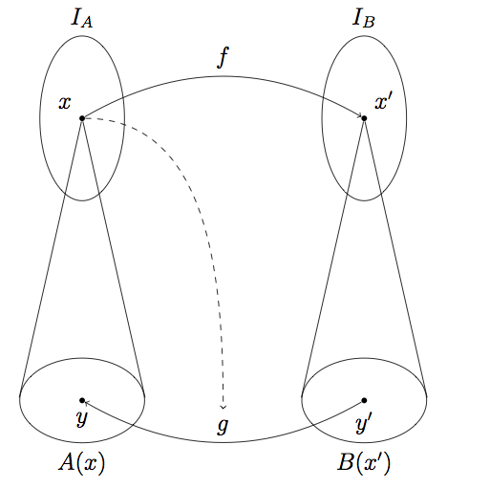
\includegraphics[width=0.7\linewidth]{img/problem_reduction}
	\caption{Graphical representation of problem reduction}
	\label{fig:problemreduction}
\end{figure}
\subsection{K-SAT*}
A variant of the k-sat problem is the $ K-SAT^* $ where between them change only the input: The $ K-SAT^* $ receive two sets of assignments $ X  $ and $ Y$ of size $ n = 2^{\frac{m}{2}} $ to respectively the first half and second half of variables where m is the number of variables and a set of clauses $ C $.\\
In order to find an assignment that satisfy $ C $ we combine each first-half assignment of X to Y, then try to check if applied to the set of clauses returns \textit{true}.\\
So the complexity of the algorithm is virtually $ O(n^2) $ on the input size, but if we substitute n in function of m (the number of variables) we obtain $ O((2^{\frac{m}{2}})^2)  = O(2^m)$. Also this problem cannot have the complexity $ O(n^{2-\varepsilon}) $ unless SETH is false.
Remember that SAT clauses are in CNF form that means:\\ \medskip
\noindent
$ (X_{1}\vee X_{2}\vee \cdots \vee X_{n})\wedge (Y_{1}\vee X_{2}\vee \cdots \vee X_{n})\wedge (X_{1}\vee Y_{2}\vee \cdots \vee X_{n})\wedge (Y_{1}\vee Y_{2}\vee \cdots \vee X_{n})\wedge \cdots \wedge (Y_{1}\vee Y_{2}\vee \cdots \vee Y_{n}). $\\
To resume in words, in CNF  variables in the clause are concatenated with OR operator while the clauses are concatenated with AND operator
\subsection{Disjoint set problem}
Given a set of sets C, the solution is 1 when exists two sets $ A,B \in C $ such that $ A \cap B = \emptyset $.
The complexity of this algorithm is $ O(|C|^2) $.
\subsection{Reduction from K-SAT* to disjoint set}
Given the set of all clauses $ C $ and X,Y respectively the assignment to the first and second half of variables, we define the collection $ S = S_1 \cup S_2 $ as follow:
\begin{center}
	$ S_1:= \{ \{t_1\} \cup \{ c : x \in X \nvDash c \,\, \forall c \in C \} \}$ \\ \medskip
	$ S_2:= \{ \{t_2\} \cup \{ c : y \in Y \nvDash c \,\, \forall c \in C \} \}$
\end{center}
$ t_1 $ and $ t_2 $ are only tokens to avoid the empty intersection between set from the same assignment.\\
To resume, if exists a good assignment in $ K-SAT^* $ then in disjoint sets should exists an empty intersection between two sets, one in $ S_1 $ and another in $ S_2 $.\\
To explain the reduction from $ K-SAT^* $ to disjoin set, a good assignment should satisfy all the clauses in K-SAT* and this thing is transposed in disjoint set with the intersection operator: given $ s_1 \in S_1 $ and $ s_2 \in S_2 $ if $ s_1 \cap s_2 \ne \emptyset$ then exists a clause not satisfied both from X and Y so the clause if false, then is not a good assignment while a good assignment should satisfy all the clauses so it should not have any clause in the intersection.
\subsection{From disjoint set to diameter computation}
Given in input a set of sets $ C $ and the variables $ X $ we can build a clique of the size of  $ X $, then add a node for each subset in $ C $ and add an edge between the node  $ c_i \in C $  and $ x_j $ if $ x_j $ appears in the set $ c_i $.\\
Then we can interpreter the diameter between $ c_i \text{ and } c_j $ in the following mode :
\begin{itemize}
	\item $ diameter(c_i, c_j) = 2  \rightarrow $  exists an intersection between $ c_i $ and $ c_j $
	\item $ diameter(c_i, c_j) = 3  \rightarrow $ not exists an intersection between $ c_i $ and $ c_j $
\end{itemize}
\begin{figure}[H]
	\centering
	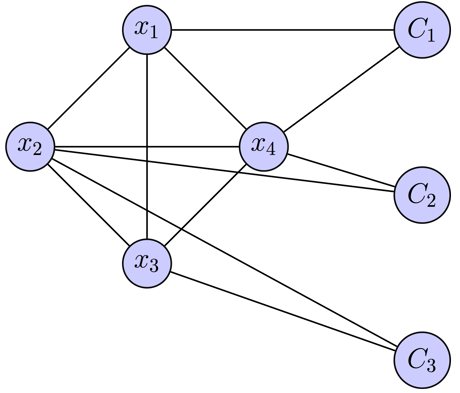
\includegraphics[width=0.5\linewidth]{img/disjoint_set_to_diameter}
	\caption{Graphical representation of reduction from disjoint sets to diameter computation}
	\label{fig:disjointsettodiameter}
\end{figure}
\subsection{Complexity of diameter computation}
With the above reductions we have demonstrated that the complexity of diameter computation cannot be in the form $ O(n^{2 - \varepsilon}) $ unless SETH is false, so the complexity of diameter cannot be lower than $ O(n^2)  $
\section{Heuristic for computing the diameter}
\subsection{BFS and diameter}
The height of BFS tree is a lower bound for computing the diameter. We can use this value also as approximation of the diameter doing many BFS from a random vertex. Below we present two methods to approximate the diameter with BFS. This approximations works well in various types of graphs (including social networks) but in other types not, for example road networks.
\subsection{2-SWEEP}
\begin{enumerate}
	\item Pick a random vertex \textit{r}
	\item Do a BFS from r
	\item Pick \textit{x}, one of the farther vertexes from r
	\item Do a BFS from \textit{x} and return the height of the BFS tree as diameter
\end{enumerate}
Complexity: $ 2 \cdot m $

\begin{figure}[H]
	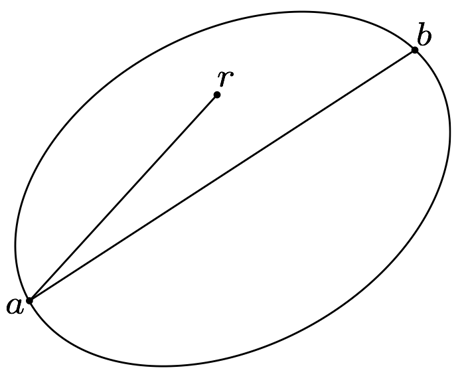
\includegraphics[width=0.4\linewidth]{img/2sweep}
	\caption{2-SWEEP graphical representation}
	\label{fig:2sweep}
\end{figure}
\subsection{4-SWEEP}
\begin{enumerate}
	\item Do a 2-SWEEP
	\item Pick one of the middle vertexes in the longest path of the 2-SWEEP
	\item Do a 2-SWEEP from that vertex
\end{enumerate}
Complexity: $ 4 \cdot m $
\section{Exact heuristic of diameter}
\subsection{Eccentricity}
The eccentricity of a vertex $ ecc(v) $ is the maximum distance between $ v $ and any other node.. In formula it is $ecc(v) = \max_{u\in V}d(u,v) $\\
We can express the diameter in terms of eccentricity: it is the maximum eccentricity among all nodes, or in formula $diameter(G) =  \max_{v \in V}ecc(v) $ 
\subsection{How heuristic works and complexity}
The intent of this exact heuristic is to find the maximum eccentricity among all nodes in order to return the diameter but the worst case doesn't change: it is always $ O(nm) $ so the reduction from $ K-SAT^* $ is valid but in the mean case this heuristic should be very effective in terms of time cost. For this purpose we use the concept of eccentricity, some definitions and a demonstration.
\subsection{Some terms}
\begin{itemize}
	\item $ F(u)  = \{v | d(u,v) = ecc(u)\}$ so the set of nodes at maximum distance from \textit{u}
	\item $ F_i(u)  = \{v | d(u,v) = i\}$ so the nodes at distance \textit{i} from \textit{u} (e.g. $ F_{ecc(u)(u) = F(u)} $ and $ F_{1}(u) = Neightbours(u) $)
	\item $ B_i(u) = \max_{z \in F_i(u)}ecc(z) $ so the maximum eccentricity between nodes at distance \textit{i} from \textit{u}
\end{itemize}
\subsection{To the upper bound}
Let's demonstrate the following assert:
For any $ 1 \leq i \leq ecc(u) $ and $ 1 \leq k < i $ and for any $ x \in F_{i-k)}(u) $ such that $ ecc(x) >2(i-1) $ there exists $ y \in F_j(u) $ such that $ d(x,y) = ecc(x) $ with $ j \geq i $.
Let's first demonstrate that $ j \geq i $:\\
First, we can do some observations:
\begin{itemize}
	\item for $ x \in F_i(u) $ or $ y \in F_i(u) $ we have that $ d(x,y) < B_i(u) $ because $ d(x,y) \leq \min\{ecc(x), ecc(y)\} \leq B_i(u) $. Remember that $ B_i(u) = max_{x \in F_i(u)}ecc(x) $
	\item for any $ 1 \leq i, j \leq ecc(u) $ and $ \forall x \in F_i(u) , y \in F_j(u) $ we have $ d(x,y) \leq i + j \leq 2 \max\{i,j\} $
\end{itemize}
With this observations we can demonstrate that $ j \geq i $. Suppose for absurd that $ i > j $, $ x \in F_{i-k}(u) $, $ ecc(x) > 2(i-1) $ and $ y_x \in F_j(u)  $ at distance $ ecc(x) $ from $ x $ we have that:
\begin{center}
	$  2(i-1)< ecc(x) = d(x,y_x) \leq 2\max\{i-k, j\} \leq 2\max\{i-k, i-1\} = 2(i-1) $ 
\end{center}
which is a contradiction so $ j \geq i $.\\
In words, it means that if a node has a eccentricity more than $ 2(i-1) $ and stay above the level \textit{i} then a node at maximum distance from \textit{x} stay below \textit{x} in the \textit{BFS tree} of \textit{u}.\\
Now let's define \textit{lb} as the maximum eccentricity below the level \textit{i} or in then we have an upper bound on $ x \in F_i(u) $ that is $  ecc(x) \leq \max\{lb, 2(i-1)\}$. We can have two cases about $ ecc(x) $ that are:
\begin{itemize}
	\item $ ecc(x) \leq 2(i-1)  \rightarrow $ is true that $ ecc(x) \leq \max\{lb, 2(i-1)\} $
	\item $ ecc(x) > 2(i-1)  \rightarrow $ in this case exists a node \textit{y} below  \textit{x} that has eccentricity greatest or equal than \textit{x}. In the latter assert we have demonstrate that if a node has eccentricity more than \textit{2(i-1)} above the level \textit{i} then exists a node \textit{y} below the level \textit{i} such that $ d(x,y) = ecc(x) $. This imply that the eccentricity of $ y $ is at minimum $ d(x,y) $ but can be also more so we can assert that $ ecc(y) \geq ecc(x) $ . In conclusion $ ecc(x)  \leq ecc(y) \leq lb $, so the dis-equation $ ecc(x) \leq \max{2(i-1), lb}  $ is respected
\end{itemize}
\subsection{The algorithm}
With the upper bound $ \max\{2(i-1), lb\} $ we can assert that if $ M > 2(i-1) $ below the level i doesn't exists a node with eccentricity more than $ lb $
so we can return $ lb $.
We can schematize the algorithm in the following steps:
\begin{enumerate}
	\item Do a BFS from a node \textit{u}
	\item Set $ i = ecc(u) \text{ and } M = B_i(u)$ 
	\item If $ M > 2(i-1) \text{ return } M; \text{ else set } i = i-1  \text{ and } M = \max\{M, B_i(u)\}$ then repeat this step while not return a value
\end{enumerate}